% ------------------------------------------------------------------------
% file `main-exercise-4-exercise-body.tex'
%   in folder `xsim/'
%
%     exercise of type `exercise' with id `4'
%
% generated by the `exercise' environment of the
%   `xsim' package v0.21 (2022/02/12)
% from source `main' on 2022/06/13 on line 6
% ------------------------------------------------------------------------
    Le diagramme à barre ci-dessous donne la répartition des notes obtenues à un contrôle de mathématiques sur 20 points par les élèves de 4 TQ.
    \begin{center}
        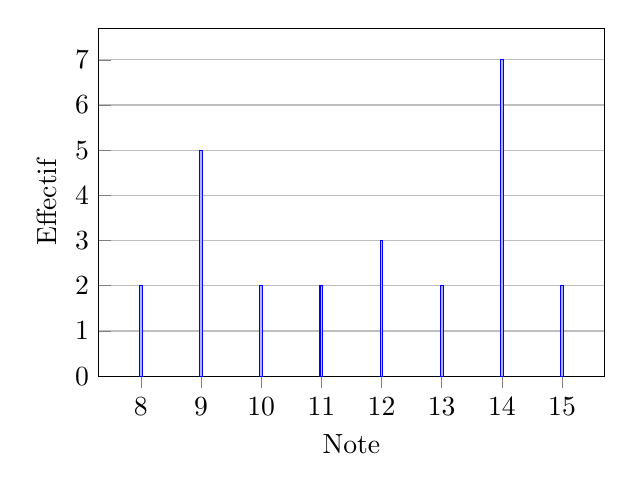
\begin{tikzpicture}
            \begin{axis} [
                ybar,
                height=6cm,
                width=8cm,
                xlabel={Note},
                ylabel={Effectif},
                ymin=0,
                xtick distance = 1,
                ytick distance = 1,
                %xtick={8,...,15},
                %ytick={1,...,7},
                ymajorgrids,
                xtick pos=bottom,
                ytick pos=left,
                bar width=1pt]
                \addplot coordinates {
                    (8,2)
                    (9,5)
                    (10,2)
                    (11,2)
                    (12,3)
                    (13,2)
                    (14,7)
                    (15,2)
                };
                \end{axis}
        \end{tikzpicture}
    \end{center}
    \begin{enumerate}
        \item Combien d'élèves y-a-t-il dans cette classe ?
        \item Quelle est la note la plus observée à ce contrôle ? En termes statistiques, comment appelle-t-on cette valeur ?
        \item Quelle est la note moyenne de la classe à ce contrôle ?
        \item Quelle est la note médiane de la classe à ce contrôle ?
        \item Si l'on considère que les élèves ont réussi s'ils ont obtenu la moitié ou plus, détermine le pourcentage de réussite de la classe.
    \end{enumerate}
